\documentclass[11pt]{article}
\usepackage[T1]{fontenc}
\usepackage{lmodern}
\pdfgentounicode=1
\pdfglyphtounicode{parenleftbig}{0028}
\pdfglyphtounicode{parenrightbig}{0029}
\pdfglyphtounicode{parenleftBig}{0028}
\pdfglyphtounicode{parenrightBig}{0029}
\pdfglyphtounicode{parenleftbigg}{0028}
\pdfglyphtounicode{parenrightbigg}{0029}
\pdfglyphtounicode{parenleftBigg}{0028}
\pdfglyphtounicode{parenrightBigg}{0029}
\usepackage[margin=1.05in]{geometry}
\usepackage{microtype}
\usepackage{amsmath,amssymb,amsthm,mathtools}
\usepackage{enumitem}
\usepackage{tikz}
\usetikzlibrary{arrows.meta,calc,decorations.pathreplacing,positioning}
\usepackage[hidelinks]{hyperref}
\hypersetup{pdftitle={A torsion-free hyperbolic group that is not residually finite},pdfauthor={OpenAI}}
\usepackage[nameinlink,capitalize,noabbrev]{cleveref}
\setlist{itemsep=3pt,topsep=5pt}
\newtheorem{theorem}{Theorem}[section]
\newtheorem{lemma}[theorem]{Lemma}
\newtheorem{proposition}[theorem]{Proposition}
\newtheorem{corollary}[theorem]{Corollary}
\theoremstyle{remark}
\newtheorem{remark}[theorem]{Remark}
\newcommand{\F}{\mathbb F}
\newcommand{\R}{\mathbb R}
\newcommand{\N}{\mathbb N}
\newcommand{\Z}{\mathbb Z}
\DeclareMathOperator{\rank}{rank}
\DeclareMathOperator{\tr}{tr}
\DeclareMathOperator{\dist}{dist}
\DeclareMathOperator{\diam}{diam}
\DeclareMathOperator{\length}{length}
\newcommand{\id}{\mathrm{id}}
\newcommand{\eps}{\varepsilon}
\numberwithin{equation}{section}
\setlength{\emergencystretch}{1em}
\title{A torsion-free hyperbolic group that is not residually finite}
\author{OpenAI}
\date{September 23, 2026}

\begin{document}
\maketitle
\begin{abstract}
We construct a torsion-free word-hyperbolic group that is not residually finite, answering the residual-finiteness question for hyperbolic groups negatively.
\end{abstract}

\section{Introduction}\label{sec:introduction}

A group $G$ is \emph{residually finite} if each nonidentity element has a nonidentity image under a homomorphism to some finite group. Equivalently, its \emph{finite residual} $R_f(G)$, the intersection of the kernels of all such homomorphisms, is trivial. A finitely generated group is \emph{word-hyperbolic} if a Cayley graph has uniformly thin geodesic triangles: there is a constant such that every point of one side is within that distance of the other two sides. The residual-finiteness question asks whether every word-hyperbolic group is residually finite.

The question belongs to the program initiated by Gromov's theory of hyperbolic groups \cite{Gromov1987}; see \cite[\S5]{AGM2009} for its formulation and consequences. It asks whether coarse negative curvature alone forces separation by finite quotients.

\begin{theorem}\label{thm:main}
There exists a torsion-free word-hyperbolic group that is not residually finite.
\end{theorem}

The group is the fundamental group of a finite Euclidean triangle complex. We prove that a member of a fixed finite family of nontrivial elements belongs to its finite residual. The argument is existential: it proves that one fixed member works for all finite quotients, without identifying which member. Thus the residual-finiteness question has a negative answer even within the torsion-free class.

The same obstruction has a classical consequence for linear representations. A group is \emph{linear over a commutative field $K$} if it admits an injective homomorphism into $\mathrm{GL}_n(K)$ for some finite $n\geq 1$.

\begin{corollary}[Finite-dimensional linear obstruction]\label{cor:nonlinear}
Let $G$ be the finitely generated torsion-free word-hyperbolic group constructed in Theorem~\ref{thm:main}. For every commutative field $K$, every integer $n\geq 1$, and every homomorphism $\rho:G\to\mathrm{GL}_n(K)$,
\[
R_f(G)\subseteq\ker\rho.
\]
Consequently, one fixed nonidentity element of $G$ is killed by all these representations, simultaneously over all such fields and dimensions. In particular, $G$ is not linear over any commutative field.
\end{corollary}

\begin{proof}
The image $\rho(G)$ is a finitely generated linear group, so it is residually finite by Malcev's theorem over commutative fields of arbitrary characteristic \cite[Theorems~VII and~VIII]{Malcev1940}; see also \cite[Introduction and \S3]{Nica2013}. If $g\in R_f(G)$ had $\rho(g)\ne 1$, a homomorphism from $\rho(G)$ to a finite group would have nonidentity value on $\rho(g)$. Its composition with $\rho$ would contradict the definition of $R_f(G)$. This proves the containment. The nonidentity finite-residual element described above is therefore killed by every such $\rho$, so none is injective.
\end{proof}

The corollary does not assert that every representation is trivial, and it makes no claim about skew fields or infinite-dimensional representations.

Nonlinearity itself was already known among hyperbolic groups. Michael Kapovich constructed an infinite hyperbolic group whose finite-dimensional representations over arbitrary fields all have finite image \cite[Theorem~8.1]{Kapovich2005}. More recently, Tholozan and Tsouvalas constructed residually finite nonlinear hyperbolic groups by amalgamating suitable finite-index subgroups of cocompact quaternionic hyperbolic lattices along maximal cyclic subgroups \cite[Theorem~1.1]{TT2025}. Thus nonlinearity alone does not exclude residual finiteness. Corollary~\ref{cor:nonlinear} records the stronger feature supplied here by a nontrivial finite residual: the kernels of all finite-dimensional representations have a common nonidentity element.

The residual-finiteness question has several equivalent class-wide formulations. Ilya Kapovich and Wise proved that all hyperbolic groups are residually finite if and only if every nontrivial hyperbolic group has a nontrivial finite quotient \cite[Theorem~1.2]{KW2000}; they also proved equivalence with the assertion that every hyperbolic group is virtually torsion-free, that is, has a torsion-free subgroup of finite index \cite[Theorem~5.1]{KW2000}. Together with Theorem~\ref{thm:main}, these equivalences imply that some nontrivial hyperbolic group has no nontrivial finite quotient, and that some hyperbolic group is not virtually torsion-free. These are conclusions about the class, not additional properties of the torsion-free group constructed here.

Agol, Groves and Manning established a further consequence of a positive answer. A subgroup is \emph{separable} if every element outside it can be distinguished from it in some finite quotient, and a subgroup of a hyperbolic group is \emph{quasiconvex} if geodesics joining its elements remain within a bounded distance of the subgroup. They proved that, if all hyperbolic groups were residually finite, then every quasiconvex subgroup of every hyperbolic group would be separable \cite[Theorem~0.1]{AGM2009}. Their filling theorem produces hyperbolic quotients that simplify intersections among conjugates of the subgroup while keeping a prescribed element outside its image \cite[Theorem~0.6]{AGM2009}. This explains the universal hypothesis: the argument needs residual finiteness of the quotient groups, not just of the initial group.

Additional geometric structure does force residual finiteness. Haglund and Wise introduced special cube complexes and proved that fundamental groups of compact virtually special cube complexes are linear; in particular, these groups are residually finite \cite[Theorem~4.4]{HW2008}. Agol proved that a word-hyperbolic group acting properly and cocompactly on a CAT(0) cube complex is virtually special \cite[Theorem~1.1]{Agol2013}. Thus a hyperbolic counterexample cannot admit such a cubulation. Strong angular-link bounds on a finite polygonal complex do not by themselves provide the cubical structure required by this theorem.

The hyperbolicity hypothesis in Agol's theorem is essential. Wise's complete square complexes, constructed in his 1996 thesis and published in \cite{Wise2007}, include compact nonpositively curved examples whose fundamental groups are not residually finite and whose universal covers are products of trees \cite[Theorem~3.8 and Main Theorem~7.5]{Wise2007}. Burger and Mozes constructed infinite finitely presented simple groups acting freely and cocompactly on products of trees \cite{BM1997}. These tree products contain Euclidean planes and are not hyperbolic. They therefore demonstrate the compatibility of nonpositive curvature with failure of residual finiteness, but not the compatibility with word hyperbolicity established here.


\paragraph{The two constraints.}
A construction must reconcile local geometric restrictions with relations that obstruct all finite quotients. Here the geometry must do more than prove hyperbolicity: it must certify that the elements used by the finite-quotient obstruction are nontrivial. The algebra also has a uniformity requirement. The finite complex, including the characteristic of the interpolation field, must be fixed before the order of a putative finite quotient is known. A rank estimate that required a larger characteristic for each quotient would not suffice.

\paragraph{The construction and its rank obstruction.}
After fixing a sufficiently large integer $r$, we choose many affine lines in a vector space over a suitably large prime field, each carrying its own marked point. A point is incident to a line when it lies on that line away from its mark. Independent sampling followed by deletion of labels on short cycles gives an incidence graph with large girth and large degree outside a small exceptional set. At each point outside the exceptional set, the incident line labels are partitioned into two blocks with Cartesian product coordinates.

For each line label $i$, the complex has an $r$-by-$r$ array of edges from one vertex $V$ to another vertex $W$. A block coordinate determines how an edge is completed to a triangle through a third vertex $O$. Shifting one coordinate by the opposite array index makes the links at $V$ and $W$ immerse in the incidence graph. The resulting link bounds ensure that a four-edge loop obtained from two distinct rows and two distinct columns of an array represents a nonidentity element. We call its group element a rectangular word; the loop alternates between $V$ and $W$.

If each of these finitely many rectangular words survived in some finite quotient, a product of the quotients would preserve all of them at once. In the regular permutation representation of this product image, each edge array becomes a block matrix of large real rank. The coordinate shifts also ensure that the sum over each Cartesian block factors through a space of small dimension. Hadamard's determinant inequality and divisibility of integer minors preserve a fixed fraction of that rank over the prime field chosen at the start, uniformly in the quotient order. Product Lagrange interpolation at the marked points then gives a tensor identity. Its left side has large rank from the edge arrays; its right side has small rank from the two local factorizations and the small exceptional set. The incompatible bounds rule out simultaneous finite separation.

\paragraph{The geometric proof.}
The group-theoretic argument uses a triangle-complex criterion whose hypotheses concern only angular lengths of closed walks in vertex links. We prove that criterion in full. Reduced planar fillings and angular Gauss--Bonnet first show that nonempty closed paths with sufficiently large turns are nontrivial; shortest representatives of free homotopy classes then exclude torsion. To obtain hyperbolicity, the strict angle excess bounds the number of original vertices inside auxiliary simple geodesic polygons in a reduced diagram. The fixed mesh converts this count into an inradius bound, and a level-arc argument gives thinness. A locally proved quasigeodesic stability estimate and a direct comparison with the Cayley graph finish the argument.

Section~\ref{sec:construction} constructs the complex and proves the rank contradiction, assuming the triangle-complex criterion stated there. Section~\ref{sec:geometry-foundations} proves the metric, filling and torsion assertions of that criterion. Section~\ref{sec:geometry-thinness} proves uniform diagram thinness and transfers it to the Cayley graph.

\section{The construction and the rank obstruction}\label{sec:construction}

\subsection{The geometric criterion}

A \emph{finite Euclidean triangle complex} will mean a finite graph with finitely many Euclidean triangles attached side-to-edge along their full boundaries, with positive compatible lengths and isometric gluings. Each closed edge and triangle is required to embed; different cells may intersect in a union of faces. The angular link at a vertex has one vertex for each incident edge germ and one edge for each triangle corner, of length equal to that corner's angle. A walk is \emph{reduced} if it has no immediate reversal, and \emph{cyclically reduced} if this also holds across its closing seam. Link distances between different components are infinite.

\begin{theorem}[Triangle complex criterion]\label{thm:triangle-complex}
Let $K$ be a connected finite Euclidean triangle complex. Suppose there is $\eta>0$ such that every nonempty cyclically reduced closed edge walk in each vertex link has angular length at least $2\pi+\eta$. Then $\pi_1(K)$ is torsion-free and word-hyperbolic.

Moreover, a nonempty closed edge path in $K$ is not nullhomotopic if every cyclic turn has link distance at least $\pi$. Here a turn compares the direction back along the arriving edge with the direction of the departing edge.
\end{theorem}

The criterion uses the classical angular-link approach to curvature;
see \cite[Theorem~II.5.2 and Lemma~II.5.6]{BH1999} for its general metric framework. We give
the complete proof of the precise statements above in
Sections~\ref{sec:geometry-foundations} and~\ref{sec:geometry-thinness},
including nontriviality for the specified turns in the original
Euclidean metric. We first use the criterion to specify the group.

\subsection{Punctured lines with few short cycles}

We need many line labels whose punctured incidence graph has large girth,
while almost every point still meets enough labels to admit the two-block
partition below. We use the probabilistic alteration method: random
sampling is followed by deletion of labels on short cycles, as in the
high-girth argument of Erd\H{o}s \cite[pp.~35--37]{Erdos1959}. The marked
line data and the exceptional-set estimates are constructed below.

Fix
\begin{equation}\label{eq:fixed-parameters}
 h=20,\qquad c=100^{-h},\qquad r\in\N\quad\text{with }cr\ge100.
\end{equation}
All limits below are as the prime $q$ tends to infinity with these constants fixed. Put $P=\F_q^h$ and $m=q^h$, and choose a subset $S\subset\F_q$ of size $\lfloor q/100\rfloor$.

\begin{lemma}\label{lem:incidence}
For all sufficiently large primes $q$, there are $N=(c+o(1))m$ affine lines $\ell_i\subset P$, indexed by a set $I$, with distinct marked points $a_i\in S^h\cap\ell_i$, and a set $E\subset P$ such that:
\begin{enumerate}[label=\textup{(\roman*)}]
\item the bipartite graph on $P\sqcup I$, with edges $z\sim i$ when $z\in\ell_i\setminus\{a_i\}$, has no cycle of length at most $12$;
\item $|I(z)|\ge4r^2$ for $z\notin E$, where
\[
 I(z)=\{i\in I:z\in\ell_i\setminus\{a_i\}\};
\]
\item $|E|=o(m)$.
\end{enumerate}
In particular we can fix such data with
\begin{equation}\label{eq:strict-budget}
 q>r,\qquad \frac{Nr}{4}>2m+r|E|.
\end{equation}
\end{lemma}

The second inequality in~\eqref{eq:strict-budget} is the numerical gap
that the final rank comparison will contradict.

\begin{proof}
Initially use every point of $S^h$ as a mark, independently choosing a uniform direction for the line through it. The number of directions is
\[
 J=\frac{q^h-1}{q-1}.
\]
For a fixed $z\in P$, each mark other than $z$ gives an incidence with probability $1/J$. Its degree is therefore binomial, with mean $\mu_z\sim cq$ uniformly in $z$ and variance at most $\mu_z$. For large $q$, $\mu_z\ge8r^2$, so the second-moment inequality gives
\[
 \Pr\bigl(|I(z)|<4r^2\bigr)
 \le \frac{\mu_z}{(\mu_z-4r^2)^2}=O(q^{-1}).
\]
The expected number of low-degree points is $O(m/q)$. By Markov's inequality, with probability tending to one there are at most $m q^{-1/2}$ such points.

For $2\le s\le6$, count simple cycles with $s$ point vertices and $s$ line labels. There are at most $m^s$ ordered choices of the points. Consecutive points force a geometric line, on which there are at most $q$ possible marks. For distinct line labels, the prescribed directions occur with probability $J^{-s}$ by independence. Choices whose mark is a forbidden punctured endpoint can only increase this upper bound. The expected number of these cycles is consequently at most
\[
 m^s q^s J^{-s}\le q^{2s},
\]
since $J\ge q^{h-1}$. This argument also allows different labels to specify the same geometric line: their random directions remain independent. Summing over $s$ shows that, with probability tending to one, the total number of cycles of length at most $12$ is at most $q^{13}$.

Choose an outcome satisfying both bounds. Delete every label appearing in one of those cycles, at most $6q^{13}$ labels, and let $E$ contain the old low-degree points and all points of the discarded lines. Deleting labels creates no cycle, and outside $E$ it changes no degree. Moreover,
\[
 |E|\le m q^{-1/2}+6q^{14}=o(m),\qquad
 N=|S|^h-O(q^{13})=(c+o(1))m.
\]
As $cr\ge100$, these estimates give~\eqref{eq:strict-budget} for large enough $q$: eventually $N/m\ge c/2$ and $r|E|/m\le1$, whereas $cr/8\ge12.5>3$.
\end{proof}

Fix the finite data in Lemma~\ref{lem:incidence} once and for all. No subsequent choice of a finite quotient will change $q$ or any of these data.

\subsection{Blocks and triangular relations}

For $z\notin E$, partition $I(z)$ into two blocks $I_b$ whose sizes factor as
\[
 |I_b|=s_b t_b,\qquad s_b,t_b\ge r.
\]
Indeed, for $d=|I(z)|\ge4r^2$, choose $n_2\in[r,2r-1]$ with $n_2\equiv d\pmod r$. Then
\[
 d=r n_1+(r+1)n_2,\qquad
 n_1=\frac{d-(r+1)n_2}{r}\ge\frac{2r^2-r+1}{r}\ge r.
\]
Use blocks of sizes $r n_1$ and $(r+1)n_2$. Index blocks at different points separately and write $p(b)$ for the point of block $b$. At points of $E$ make no blocks. For each block fix a bijection
\begin{equation}\label{eq:block-coordinates}
 i\longmapsto\bigl(\alpha_b(i),\beta_b(i)\bigr)
 \in\Z/s_b\Z\times\Z/t_b\Z.
\end{equation}

Let $[r]=\{0,\ldots,r-1\}$. Form a complex $K$ with vertices $O,V,W$ and edges
\[
\begin{array}{ll}
 x_{iuv}:V\longrightarrow W & (i\in I,\ u,v\in[r]),\\[2pt]
 L_{b,u,j}:O\longrightarrow V & (u\in[r],\ j\in\Z/s_b\Z),\\[2pt]
 R_{b,v,k}:O\longrightarrow W & (v\in[r],\ k\in\Z/t_b\Z).
\end{array}
\]
For every $b$, $i\in I_b$, and $u,v\in[r]$, attach a triangle with sides
\begin{equation}\label{eq:triangle-sides}
 x_{iuv},\qquad L_{b,u,\alpha_b(i)+v},\qquad
 R_{b,v,\beta_b(i)+u}.
\end{equation}
Give each triangle angles $3\pi/5,\pi/5,\pi/5$ at $O,V,W$, respectively, using one fixed shape. All edge lengths are compatible; assign the same appropriate lengths to unused edges as well. Closed cells embed because the three vertices of every triangle are distinct. There are regular points and hence blocks, so $K$ is connected.

Figure~\ref{fig:construction-triangle} shows one of these triangles.
The larger angle at $O$ will control the four-edge cycles in its link;
the smaller angles at $V$ and $W$ will be paired with the large girth of
the incidence graph.

\begin{figure}[htbp]
\centering
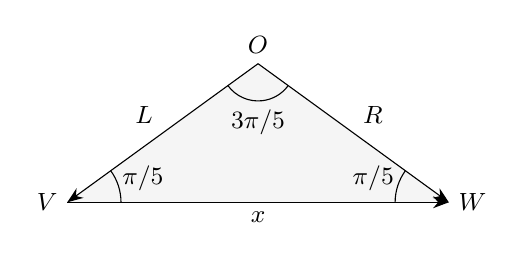
\begin{tikzpicture}[scale=1.1, every node/.style={font=\small}]
  \coordinate (O) at (0,1.6);
  \coordinate (V) at (-2.20221,0);
  \coordinate (W) at (2.20221,0);
  \fill[gray!8] (O)--(V)--(W)--cycle;
  \draw[-{Stealth[length=2mm]}] (O)--node[above left] {$L$} (V);
  \draw[-{Stealth[length=2mm]}] (O)--node[above right] {$R$} (W);
  \draw[-{Stealth[length=2mm]}] (V)--node[below] {$x$} (W);
  \draw (O) ++(216:.43) arc[start angle=216,end angle=324,radius=.43];
  \draw (V) ++(0:.62) arc[start angle=0,end angle=36,radius=.62];
  \draw (W) ++(144:.62) arc[start angle=144,end angle=180,radius=.62];
  \node at (0,.92) {$3\pi/5$};
  \node at (-1.33,.28) {$\pi/5$};
  \node at (1.33,.28) {$\pi/5$};
  \node[above] at (O) {$O$};
  \node[left] at (V) {$V$};
  \node[right] at (W) {$W$};
\end{tikzpicture}
\caption{One attached triangle, with $L,R,x$ abbreviating the indexed
edges in \eqref{eq:triangle-sides}. The oriented boundary is
$LxR^{-1}$. Many distinct edges and triangles share the same three
vertices in $K$; the picture shows only one triangle.}
\label{fig:construction-triangle}
\end{figure}

\begin{lemma}\label{lem:links}
The complex $K$ satisfies Theorem~\ref{thm:triangle-complex} with $\eta=2\pi/5$. At either $V$ or $W$, the link distance between distinct $x$-directions with the same label $i$ is at least $14\pi/5$, or is infinite.
\end{lemma}

\begin{proof}
At $O$, each block gives a complete bipartite link on its $L$- and $R$-directions. For fixed $u,v,j,k$, the equations
\[
 \alpha_b(i)=j-v,\qquad \beta_b(i)=k-u
\]
specify exactly one $i\in I_b$. Thus there is one link edge per pair of directions, and every nonempty cyclically reduced closed walk has at least four edges. Its angular length is at least $12\pi/5$.

Project the link at $V$ to the incidence graph of Lemma~\ref{lem:incidence} by sending an $x_{iuv}$-direction to $i$ and an $L_{b,u,j}$-direction to $p(b)$. This map is locally injective on edges. At $x_{iuv}$ there is at most one incident triangle over any point $z$, because $i$ lies in at most one block at $z$. At $L_{b,u,j}$, fixing $i$ determines at most one $v\in[r]$ from $j=\alpha_b(i)+v$, since $s_b\ge r$. The link at $W$ has the same property using $t_b\ge r$ and the $R$-directions. Every cyclically reduced link walk therefore has a reduced image and at least $14$ edges, of angular length at least $14\pi/5$.

A reduced path between distinct $x$-directions with the same $i$ projects to a positive closed walk reduced at every internal vertex. It need not be reduced at its closing seam, but it still contains a simple cycle: choose a shortest positive subwalk with equal endpoints. A subwalk of length two would be an internal reversal, and one of length one is impossible in this graph. The path therefore has at least $14$ edges. A shortest link path is reduced, proving the distance assertion.
\end{proof}

Set $G=\pi_1(K,O)$. Theorem~\ref{thm:triangle-complex} and Lemma~\ref{lem:links} show that $G$ is torsion-free and word-hyperbolic. It remains to exclude residual finiteness.

Choose a path from $O$ to each vertex and associate to an oriented edge $e$ the based loop given by the path to its initial vertex, then $e$, then the reverse of the path to its terminal vertex. Write its element as $g_e$, using multiplication in path order, and abbreviate $g_{iuv}=g_{x_{iuv}}$. The triangles give
\begin{equation}\label{eq:group-factorization}
 g_{iuv}=g_{L_{b,u,\alpha_b(i)+v}}^{-1}
               g_{R_{b,v,\beta_b(i)+u}}\qquad(i\in I_b).
\end{equation}
Furthermore,
\begin{equation}\label{eq:rectangles}
 g_{iuv}g_{iu'v}^{-1}g_{iu'v'}g_{iuv'}^{-1}\ne1
 \qquad(u\ne u',\ v\ne v').
\end{equation}
Indeed, after cancelling the chosen connecting paths this word is conjugate to a closed four-edge path. Each of its four turns compares distinct same-$i$ directions in a link at $V$ or $W$, and so has distance at least $\pi$ by Lemma~\ref{lem:links}. The closed-path assertion of Theorem~\ref{thm:triangle-complex} applies.

Let $\mathcal R\subset G$ be the finite set of rectangular words in
\eqref{eq:rectangles}, with $i\in I$, $u\ne u'$ and $v\ne v'$ in $[r]$.
We have proved $1\notin\mathcal R$. The remaining argument shows that
no finite quotient can keep every member of $\mathcal R$ nonidentity.

\subsection{Rank over the reals and over a fixed prime field}

The following elementary observation makes it possible to choose the characteristic independently of a prospective finite quotient.

\begin{lemma}[Rank under reduction]\label{lem:rank-reduction}
Let $M$ be an integer matrix whose rows have Euclidean norm at most $\sqrt r$, where $r\ge1$. For every prime $q>r$,
\[
 \rank_{\F_q}M\ge\tfrac12\rank_{\R}M.
\]
\end{lemma}

\begin{proof}
Let $d=\rank_{\R}M$; the assertion is immediate for $d=0$. A nonzero $d\times d$ minor $B$ has
\[
 1\le|\det B|\le r^{d/2},
\]
by Hadamard's determinant inequality, obtained by orthogonalizing its rows. If $d'=\rank_{\F_q}B$, choose $d'$ rows spanning its row space modulo $q$. Subtract integer lifts of their linear combinations from the other rows. These determinant-preserving operations make $d-d'$ rows divisible by $q$, whence
\[
 q^{d-d'}\mid\det B,\qquad q^{d-d'}\le r^{d/2}.
\]
Since $q>r$, we obtain $d'\ge d/2$, as required.
\end{proof}

Suppose, for a contradiction, that a finite quotient $Q$ of $G$ keeps every member of $\mathcal R$ nonidentity. Put $D=|Q|$. For an element $g\in G$, let $U(g)$ be its $D\times D$ regular permutation matrix on $Q$, using left multiplication and column vectors. Thus $U$ is a homomorphism and $U(g)^{\mathsf T}=U(g^{-1})$.

For $i\in I$ form the integer matrix of $D\times D$ blocks
\begin{equation}\label{eq:Yi}
 Y_i=\bigl(U(g_{iuv})\bigr)_{u,v\in[r]}.
\end{equation}
The real trace of the regular permutation of a nonidentity element is zero, whereas the identity has trace $D$. Expanding in blocks gives
\begin{align}
 \tr(Y_iY_i^{\mathsf T})&=r^2D,\label{eq:trace-first}\\
 \tr\bigl((Y_iY_i^{\mathsf T})^2\bigr)&=(2r^3-r^2)D.\label{eq:trace-second}
\end{align}
In the second expansion, a term is the trace of
\[
 U\bigl(g_{iuv}g_{iu'v}^{-1}g_{iu'v'}g_{iuv'}^{-1}\bigr).
\]
It equals $D$ when $u=u'$ or $v=v'$, and is zero otherwise by~\eqref{eq:rectangles}. There are $2r^3-r^2$ degenerate index choices.

Cauchy--Schwarz on the positive eigenvalues of $Y_iY_i^{\mathsf T}$ now gives
\[
 \rank_{\R}Y_i\ge
 \frac{r^4D^2}{(2r^3-r^2)D}
 =\frac{r^2D}{2r-1}\ge\frac{rD}{2}.
\]
Each row of $Y_i$ has exactly $r$ unit entries. Lemma~\ref{lem:rank-reduction} therefore yields
\begin{equation}\label{eq:rank-lower}
 \rank_{\F_q}Y_i\ge\frac{rD}{4}.
\end{equation}
There is no restriction on $D$, and in particular no assumption that $q$ does not divide $D$.

\subsection{Local factorizations and the global certificate}

We will express the direct sum of the high-rank matrices $Y_i$ as a sum
of terms with small total rank. The triangle relations give the local
rank bounds; interpolation supplies weights that combine them.

Work henceforth over $\F_q$, and put
\[
 Z(z)=\sum_{i\in I(z)}Y_i\qquad(z\in P).
\]
At a regular point $z\notin E$, each of its two blocks satisfies
\begin{equation}\label{eq:matrix-factorization}
 \sum_{i\in I_b}Y_i
 =\left(\sum_{j\in\Z/s_b\Z}U(g_{L_{b,u,j}}^{-1})\right)_{u\in[r]}
  \left(\sum_{k\in\Z/t_b\Z}U(g_{R_{b,v,k}})\right)_{v\in[r]}.
\end{equation}
The first factor is a block column and the second a block row. For each fixed $u,v$, the shifted coordinates in~\eqref{eq:group-factorization} run through all pairs $(j,k)$ exactly once. The two complete sums are independent of the opposite block index, so~\eqref{eq:matrix-factorization} is a factorization of the whole matrix, with inner dimension $D$. The order of the factors is preserved; no commutativity is used. Hence
\begin{equation}\label{eq:rank-upper}
 \rank Z(z)\le
 \begin{cases}
 2D,&z\notin E,\\
 rD,&z\in E.
 \end{cases}
\end{equation}
For exceptional points we use the ambient matrix dimension. Their incidences have not been deleted from $I(z)$.

We now construct scalar matrix weights whose sum over a punctured line
isolates that line's label. For each $i\in I$, product Lagrange interpolation on $S^h$ supplies a polynomial $f_i$ of total degree at most $h(|S|-1)$ with
\[
 f_i(a_{i'})=\begin{cases}1,&i=i',\\0,&i\ne i'.\end{cases}
\]
Explicitly, for $a_i=(a_{i1},\ldots,a_{ih})$, take
\[
 f_i(X_1,\ldots,X_h)=
 \prod_{t=1}^h\ \prod_{a\in S\setminus\{a_{it}\}}
 \frac{X_t-a}{a_{it}-a}.
\]
Let $f$ be the $N$-entry column of these polynomials and set $H(z)=f(z)f(z)^{\mathsf T}$, an $N\times N$ matrix. The matrices $Z(z)$ have size $rD\times rD$. Then $\rank H(z)\le1$ and $H(a_i)=E_{ii}$, the $i$th diagonal matrix unit.

Every entry of $H$ restricts to a polynomial of degree at most $2h(|S|-1)<q-1$ on an affine line. The finite-field power-sum identity says that such a polynomial sums to zero over $\F_q$. Indeed the constant sum is $q=0$, and for $1\le j<q-1$ there is $a\in\F_q^\times$ with $a^j\ne1$, by the polynomial root bound. Multiplying the sum of $T^j$ by $a^j$ permutes its summands and forces that sum to vanish. Thus
\begin{equation}\label{eq:line-certificate}
 \sum_{z:\,i\in I(z)}H(z)=-H(a_i)=-E_{ii}.
\end{equation}
Only the line's own mark is omitted. Other marks on that line, if any, remain in the sum.

Exchanging finite sums in~\eqref{eq:line-certificate} gives
\begin{equation}\label{eq:tensor-certificate}
 -\bigoplus_{i\in I}Y_i
 =-\sum_{i\in I}E_{ii}\otimes Y_i
 =\sum_{z\in P}H(z)\otimes Z(z).
\end{equation}
The rank of the left side is at least $NrD/4$ by~\eqref{eq:rank-lower}. The image of $H(z)\otimes Z(z)$ lies in the tensor product of the two images, of dimension at most $\rank Z(z)$. Rank subadditivity and~\eqref{eq:rank-upper} therefore give
\[
 \frac{NrD}{4}\le 2mD+r|E|D.
\]
After cancellation of the positive integer $D$, this contradicts~\eqref{eq:strict-budget}.
Thus no finite quotient preserves all of
$\mathcal R$. If each $w\in\mathcal R$ had a nonidentity image in some
finite group, the product of those finitely many maps, followed by taking
its image, would give precisely such a quotient. Consequently there is
one fixed $w\in\mathcal R$ whose image is the identity under every
homomorphism from $G$ to a finite group. Since $w\ne1$ in $G$, the finite
residual of $G$ is nontrivial. This proves Theorem~\ref{thm:main}, subject
only to the geometric criterion proved next.

\section{Metrics, planar fillings, and torsion}
\label{sec:geometry-foundations}

We begin the proof of Theorem~\ref{thm:triangle-complex}. Here we establish
two conclusions: nonempty closed edge paths with cyclic
turns of link distance at least $\pi$ are nontrivial, and $\pi_1(K)$ is
torsion-free. Reduced planar fillings turn angular-link bounds into a
curvature obstruction; shortest free loops turn that obstruction into
torsion-freeness. Uniform thinness and the passage to the Cayley graph
are proved in Section~\ref{sec:geometry-thinness}.

Throughout this section, $K$ is the finite Euclidean triangle complex in that theorem;
``original'' refers to its cells before subdivision. A link is regarded as a
metric graph, with the length of each edge equal to the angle of its corner.
As in Section~\ref{sec:construction}, a closed link walk is
\emph{cyclically reduced} if consecutive edges, including the last
and first, are never mutual reverses.

\subsection{Subdivisions and shortest paths}

Barycentrically subdivide $K$. This gives a genuine simplicial complex:
its vertices are the original cells, and its simplices are their strict
inclusion chains. In particular, distinct parallel original edges have
distinct barycenters, and triangles meeting in several faces cause no
identifications within a simplex. Realize the subdivision by straight
segments in each Euclidean triangle. At an original vertex this only
subdivides the angular link, preserving its metric. At a point in the
interior of an original triangle, the link is a circle of length $2\pi$.
At a point in the interior of an original edge, its two tangent directions
are joined by one path of length $\pi$ for each incident triangle. If there
are no incident triangles, the two directions are isolated. Thus every
nonempty cyclically reduced closed walk at a new vertex has length
at least $2\pi$; at an original vertex the stronger lower bound
$2\pi+\eta$ remains valid.

These statements hold after any further compatible Euclidean subdivision.
For the later uniform estimates we will return to the fixed barycentric
subdivision, in which each small triangle has an original vertex among its
vertices.

The intrinsic distance on a connected finite Euclidean triangle complex
is the infimum of the lengths of finite paths made of straight segments
in its cells. We use the same convention on the planar complexes below,
which may have edges belonging to no triangle and pieces meeting only at
a vertex.

\begin{lemma}[Metric preliminaries]
\label{lem:finite-geodesics}
This intrinsic distance is a metric inducing the complex topology. The
complex is compact, any two points are joined by a shortest path, and every
constant-speed local geodesic has finitely many straight pieces on a compact
parameter interval. The last assertion also holds for closed local geodesics.
If such a path lies in the edges of a Euclidean subdivision, the link
distance at each of its turns is at least $\pi$.
\end{lemma}

\begin{proof}
At a point $x$, cut the incident cells into sectors centered at $x$ and
choose $\rho>0$ smaller than the distances to their nonincident faces.
The resulting truncated star consists of finitely many sectors and,
possibly, isolated radial intervals, glued along radial sides. Its radial
coordinate $r$ agrees across these gluings, and changes by at most the
length of a polygonal path. In particular, a path from $x$ leaving the
star has length at least $\rho$. For a point of radius $r<\rho$, the radial
segment has length $r$; any shorter competitor stays in the star and has
length at least $r$. Hence its distance from $x$ is exactly $r$.

This description proves positivity of the distance and identifies the
small metric neighborhoods with the usual star neighborhoods. The metric
therefore induces the complex topology. It also supplies contracting
neighborhoods, by radial contraction. Finiteness of the complex gives
compactness. Parameterize a sequence of polygonal paths whose lengths
decrease to the distance between two fixed points proportionally to
arclength on $[0,1]$. Their speeds are uniformly bounded. Compactness and
equicontinuity give a uniformly convergent subsequence: this follows, for
example, by a diagonal choice on a countable dense subset of $[0,1]$ and
then the common modulus of continuity. For every fixed partition, the
sum of distances between successive points passes to the limit. Taking
the supremum over partitions shows that the limiting path has length at
most the limiting lengths. Since every path has length at least the
distance of its endpoints, this is a shortest path.

Consider now a sufficiently short unit-speed minimizing arc starting at
$x$. Its image lies in the truncated star, and the preceding radial
formula gives $r(t)=t$. At positive radius, its direction varies
continuously in the finite graph of directions of the star. If that
direction were nonconstant, it would traverse an interval in the interior
of one of the graph's edges: a continuous map with image in the finite
set of junctions and isolated directions is constant. Choose a subarc
inside the corresponding open sector whose endpoint directions differ.
The sector is locally Euclidean, and the length of this subarc is at
least the Euclidean distance of its endpoints, which is strictly larger
than the difference of their radii. This contradicts $r(t)=t$ and
unit speed. Thus the arc is radial and straight in one sector or radial
edge. Apply the argument on both sides of each parameter value of a local
geodesic. A finite subcover of its compact parameter interval gives
finitely many straight pieces. For a closed curve use the parameter
circle, so this also includes its seam.

Finally, an angular path of length less than $\pi$ between the incoming
backward direction and the outgoing direction yields a shorter chord.
Indeed, take two nearby points at equal distance from the turn, unfold
the consecutive sectors traversed by that angular path, and join the
points by the straight chord in the sector of total angle less than
$\pi$. Its length is less than the sum of the two radial lengths.
The chord maps back to a path in the complex; the unfolded sector need
not be embedded there. This contradicts local minimality.
\end{proof}

\subsection{Reduced planar fillings with a prescribed boundary}

A \emph{planar diagram} will mean a finite connected complex embedded
topologically in the plane, with edges and triangular faces, such that
every bounded complementary face of its graph is filled by a triangle.
Its exterior walk goes once around the unbounded complementary face,
counting incidences: it can repeat vertices, and traverses an edge with
no incident triangle twice. The embedding specifies the cyclic orders;
the Euclidean metrics on the triangles need not come from this planar
embedding.

\begin{lemma}[Reduced fillings]
\label{lem:reduced-diagrams}
Let $S$ be the barycentric subdivision of $K$, or a further compatible
Euclidean simplicial subdivision. Every prescribed nonempty
nullhomotopic closed edge path in $S$ is the exterior walk of a planar
diagram $\Delta$ with a map $\Delta\to S$ that maps each edge and triangle
isometrically onto an edge and triangle, respectively. Each triangle of
$\Delta$ has three distinct vertices and edges. At every interior
vertex of $\Delta$, the cyclic sequence of corners maps to a nonempty
cyclically reduced closed walk in the target link.
Every edge loop in $\Delta$ contracts in $\Delta$.
\end{lemma}

\begin{proof}
We form a labelled picture from a disk filling, minimize its number of
nodes, erase components disjoint from the boundary, and take the planar
dual, retaining the prescribed boundary word, including spurs.
Start with a continuous filling of the path by a disk,
with its boundary mapped linearly along each prescribed edge traversal.
Mark all boundary breakpoints. Barycentric coordinates for the vertices
of the genuine simplicial complex $S$, extended by zero outside their
stars, are continuous. Triangulate the disk sufficiently finely,
respecting the marked boundary points, that each coordinate varies by
less than $1/4$ on each domain triangle. Label a domain vertex by a
target vertex of largest coordinate in its image. This coordinate is
at least $1/3$, because $S$ has dimension at most two. At every point of
a domain triangle all its chosen labels therefore have positive
coordinate, since $1/3-1/4>0$. They belong to one target simplex.
Extending the labels linearly gives a simplicial map, allowing collapsed
edges and triangles.

Along each prescribed boundary edge the only possible labels are its
two endpoints. The boundary parametrization is monotone along that edge,
so the largest-coordinate label changes from the initial endpoint to the
terminal endpoint exactly once; either choice at a midpoint tie has this
property. Consequently the noncollapsed boundary steps are exactly the
prescribed edge word, in its prescribed order. The same argument on an
interval or circle shows that every loop based at a vertex has a based
edge-loop representative: the original map and its approximation
interpolate inside common target simplices, fixing the basepoint.

For the simplicial filling, draw the inverse images of ties for the
largest target coordinate. Inside a domain triangle mapped onto a
target triangle they are three arcs meeting at a trivalent node.
Inside a triangle mapped to an edge they form one separating arc, and
inside a triangle mapped to a vertex they are absent. Suppress all bends
of valence two. We obtain a finite polygonal \emph{picture}: its regions
are labelled by target vertices; an arc separates distinct labels that
span a target edge; and the three labels at every interior trivalent
node span a target triangle. Its boundary endpoints are leaves, one for
each letter of the prescribed edge word. Components disjoint from the
boundary, including circles, are allowed.

Among all labelled pictures with these local rules and these boundary
data, choose one with the fewest trivalent nodes. No arc can join two
nodes labelled by the same target triangle. To see this, let the labels
on its two sides be $a,b$, and let $d$ be the third vertex of that
triangle. The selected arc and its endpoints form an embedded interval.
A sufficiently thin regular neighborhood is a disk meeting the four
other incident half-arcs in four distinct boundary slots
(Figure~\ref{fig:picture-cancellation}). The two slots
on the $a$-side both separate $a$ from $d$; those on the $b$-side both
separate $b$ from $d$. Erase the two nodes and the intervening arc and
join each of these two pairs along its side of the neighborhood, with
label $d$ between the new arcs. The new arcs do not cross, and every
boundary label of the neighborhood is unchanged. This gives a picture
with two fewer nodes.

The argument is unaffected if some of the four half-arcs reconnect
outside the neighborhood: their slots remain distinct and their outside
continuations retain the same labels. In particular, an additional arc
between the nodes merely makes a lens outside the chosen neighborhood.
An arc cannot join a node to itself, since the three incident arcs there
have three different target-edge labels.

\begin{figure}[htbp]
\centering
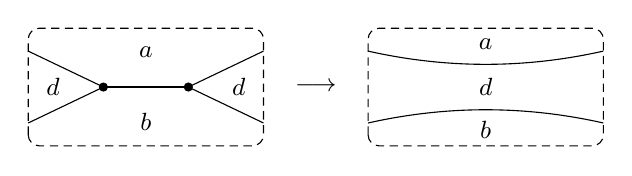
\begin{tikzpicture}[scale=.83, every node/.style={font=\small}]
  \begin{scope}[xshift=-2.6cm]
    \draw[densely dashed, rounded corners=4pt] (-1.8,-.9) rectangle (1.8,.9);
    \draw (-1.8,.55)--(-.65,0)--(-1.8,-.55);
    \draw (1.8,.55)--(.65,0)--(1.8,-.55);
    \draw (-.65,0)--(.65,0);
    \fill (-.65,0) circle (2pt);
    \fill (.65,0) circle (2pt);
    \node at (0,.53) {$a$};
    \node at (0,-.53) {$b$};
    \node at (-1.42,0) {$d$};
    \node at (1.42,0) {$d$};
  \end{scope}
  \node at (0,0) {$\longrightarrow$};
  \begin{scope}[xshift=2.6cm]
    \draw[densely dashed, rounded corners=4pt] (-1.8,-.9) rectangle (1.8,.9);
    \draw (-1.8,.55) .. controls (-.6,.28) and (.6,.28) .. (1.8,.55);
    \draw (-1.8,-.55) .. controls (-.6,-.28) and (.6,-.28) .. (1.8,-.55);
    \node at (0,.65) {$a$};
    \node at (0,-.65) {$b$};
    \node at (0,0) {$d$};
  \end{scope}
\end{tikzpicture}
\caption{Cancellation inside a thin disk neighborhood. Its four slots
and all boundary labels are preserved, regardless of reconnections
outside the disk.}
\label{fig:picture-cancellation}
\end{figure}

Next erase every component of the picture that misses the boundary.
Here the existence of consistent region labels deserves attention.
The retained picture together with the boundary circle is a connected
polygonal graph $H$. Each of its inside regions is a disk interior whose
boundary is a walk, possibly with repeated vertices and edges. One way
to see this is to build $H$ from the boundary circle: first attach tree
edges reaching all its other vertices, which slit disk regions, and then
add the remaining arcs, each of which splits a disk region into two.
Cutting apart repeated boundary incidences gives a polygon for each
region, with its interior embedded in the original disk.

Take a thin regular neighborhood of $H$ missing all erased components,
which are finitely many compact sets disjoint from $H$. For each inside
region, one connected curve in the boundary of this neighborhood follows
its entire boundary walk on the region side. In particular it follows
the two sides of a bridge separately, and follows every incidence at a
repeated vertex. This curve crosses no arc of the old picture and so lies
in one old labelled region. All labels prescribed along the boundary
incidences of the retained region are therefore equal. Extend that label
over the region. Erasing these components cannot increase the number of nodes,
so minimality is preserved.

Now construct its dual. Put a vertex in each region, and in that
region's polygon join this vertex to the midpoint of each incident arc
side by radii disjoint except at the vertex. Join the radii across the
arcs to obtain dual edges. Around each trivalent node the three
consecutive pairs of radii enclose a triangular region. Its three dual
vertices are distinct, since their region labels are the three distinct
vertices of a target triangle. The dual graph is connected, as can be
seen by taking paths between regions transverse to the picture arcs.

An Euler count verifies that these triangles fill all its bounded
faces. Let $E,N,L$ denote the numbers of retained picture arcs, trivalent
nodes, and boundary leaves. The boundary word is nonempty, so $L>0$.
Adjoining the circle subdivided at the leaves gives a connected planar
graph with $N+L$ vertices and $E+L$ edges. If $F$ is its number of inside
regions, Euler's formula gives
\[
 (N+L)-(E+L)+(F+1)=2,
 \qquad F=E-N+1.
\]
The dual graph has $F$ vertices and $E$ edges, hence exactly
$E-F+1=N$ bounded complementary faces. The $N$ disjoint triangular
regions already constructed exhaust them. Filling these triangles gives
the required planar diagram with no holes. The labels define its map
to $S$; assign each edge and triangle the metric of its image.

At a boundary leaf of the picture, its dual edge has an exterior
incidence. The interval between two successive leaves identifies the
corresponding sector at a region vertex. Following the original boundary
circle thus follows the dual exterior walk in exactly the prescribed
order. In particular, a picture arc with both endpoints on the boundary
produces an edge with no incident triangle, encountered twice. If there
are no nodes, the dual has $E+1$ vertices and $E$ edges and is a tree;
its spurs are still part of the exterior walk.

At an interior dual vertex, an immediate reversal of two successive
link edges would mean that the corresponding adjacent triangles map
to the same target triangle. Their picture nodes are joined by the
arc dual to their shared edge, contradicting minimality. This includes
the last and first corners in the cyclic order. Finally, every simple
edge circuit in the diagram bounds its filled planar disk. Any closed
edge walk splits at repeated vertices into such circuits and cancellable
backtracks, so every edge loop is nullhomotopic in the diagram.
\end{proof}

\subsection{Angular curvature and nontrivial closed paths}

Reduced fillings now let us compare the angular length of a target link
walk with the angles around a diagram vertex. Summing these angles will
show that a nullhomotopic boundary cannot have all its cyclic turns at
least $\pi$.

For a vertex $y$ of a diagram from Lemma~\ref{lem:reduced-diagrams}, let
$\theta_y$ be the sum of its incident triangle angles and let $n_y$ be
the number of exterior sectors there, equivalently its number of visits
in the exterior walk. Thus $n_y=0$ at an interior vertex. The reduced
link condition and the subdivision observations give
\[
 \theta_y\ge 2\pi \quad(n_y=0),\qquad
 \theta_y\ge 2\pi+\eta
 \quad\text{if also $y$ maps to an original vertex of $K$.}
\]

If $v,e,t$ count the vertices, edges, and triangles, planarity without
holes gives $v-e+t=1$. Counting exterior edge incidences, including both
sides of an edge belonging to no triangle, gives
$\sum_y n_y=2e-3t$. As each triangle has angle sum $\pi$, it follows that
\begin{equation}
 \sum_y\bigl((2-n_y)\pi-\theta_y\bigr)
 =2\pi v-\pi(2e-3t)-\pi t
 =2\pi.
 \label{eq:gauss-bonnet}
\end{equation}
This angular Gauss--Bonnet identity counts exterior visits with
multiplicity; it does not require a simple boundary.

\pagebreak[0]
\begin{samepage}
\begin{proposition}[Closed paths]
\label{prop:closed-paths}
In $K$, or any compatible Euclidean simplicial subdivision of it, a
nonempty closed edge path whose every cyclic turn has link distance at
least $\pi$ is not nullhomotopic.
\end{proposition}
\end{samepage}

\begin{proof}
First work in a simplicial subdivision and suppose such a path were
nullhomotopic. Apply Lemma~\ref{lem:reduced-diagrams}. At an interior
vertex the summand in \eqref{eq:gauss-bonnet} is nonpositive. At a vertex
with $n_y=1$, its consecutive interior corners supply a link path between
the two boundary directions, of length $\theta_y$. The prescribed turn
therefore implies $\theta_y\ge\pi$, so this summand too is nonpositive.
The only possibility with no intervening corner is a tip of a naked
edge: its two directions coincide, giving turn distance zero, and is
excluded by the hypothesis. If $n_y\ge2$, then
$(2-n_y)\pi-\theta_y\le0$ without any further condition. Thus every
summand is nonpositive, contradicting \eqref{eq:gauss-bonnet}.

For a path in the original complex, pass to the barycentric subdivision.
Its old turn distances are unchanged. At a new point along an original
edge, the straight-through directions have link distance $\pi$ when
the edge belongs to a triangle, and infinite distance otherwise.
The subdivided path therefore satisfies the same hypothesis.
\end{proof}

\subsection{Shortest free loops and torsion}

The closed-path obstruction applies to every positive repetition of a
closed local geodesic. We will show that each nontrivial free homotopy
class contains such a geodesic, so no nontrivial element can have finite
order.

\begin{proposition}
\label{prop:no-torsion}
The group $\pi_1(K)$ is torsion-free.
\end{proposition}

\begin{proof}
We first justify a shortest-loop argument using only the local metric
description. The contracting star neighborhoods and compactness give
$\epsilon>0$ such that every ball of radius $5\epsilon$ is contained in
a neighborhood contractible in $K$. Indeed, take a finite cover by
contracting stars with Lebesgue number $a>0$, and choose
$\epsilon<a/20$, so each such ball has diameter less than $a$.
Every loop of length less than $5\epsilon$ is contained in such a ball
about one of its points and is nullhomotopic.

Uniformly $\epsilon$-close loops are freely homotopic. To verify this,
partition their common parameter circle so that on each interval the
first loop stays within $\epsilon$ of its starting point. Join the
corresponding partition points by shortest paths, of length less than
$\epsilon$, using Lemma~\ref{lem:finite-geodesics} and the same connector
at the cyclic seam. On each interval the
second loop stays within $2\epsilon$ of that same starting point, by
pointwise closeness; no speed bound on the second loop is needed. The
two subarcs and the two connectors form a quadrilateral loop contained
in a ball of radius $3\epsilon$. It contracts in the chosen larger
neighborhood. Fill each such quadrilateral and glue along the shared
connectors to obtain an annular homotopy.

Let $g\ne1$ in $\pi_1(K)$ and consider the free homotopy class of a loop
representing $g$. It does not contain a constant loop. It has rectifiable
representatives by the edge approximation used in
Lemma~\ref{lem:reduced-diagrams}, and their lengths have infimum
$\ell\ge5\epsilon$. Parameterize a minimizing sequence proportionally
to arclength on the parameter circle. Its speeds are bounded, so the
compactness argument of Lemma~\ref{lem:finite-geodesics} supplies a
uniformly convergent subsequence. The limit lies in the same free
homotopy class by the preceding closeness argument. Lower
semicontinuity of length shows that its length is $\ell$.

Parameterize this minimizer by arclength. It is a local geodesic,
including across the cyclic seam. Otherwise some subarc of length
less than $\epsilon$ could be replaced by a shorter shortest path
with the same endpoints. Both paths lie within $\epsilon$ of the
initial endpoint, so the loop formed by them contracts in the chosen
neighborhood. The replacement preserves the free homotopy class and
shortens its representative, a contradiction.

By Lemma~\ref{lem:finite-geodesics}, this closed local geodesic has
finitely many straight pieces. Insert them into a finite compatible
Euclidean subdivision of the barycentric triangulation. First mark all
curve-piece endpoints on its edges, including edges belonging to no
triangle. In each triangle, insert their finitely many distinct supporting lines and mark
their endpoints, intersections, and ends of overlaps. The lines cut
the triangle into convex polygons. On each shared edge, collect all
its marks, including those supplied by its incident triangles, and impose this
finite set on every incident triangle. Cone each convex polygon from
an interior point to the consecutive marked points of its boundary.
This introduces no further boundary marks, so it gives a compatible,
genuine finite Euclidean triangulation containing the curve in its
edges. The
subdivision preserves the angular links and their lower bounds, as
described at the start of this section. Every turn of the curve has
link distance at least $\pi$ by local geodesicity.

If $g$ had finite order, a positive repetition of this curve would be
nullhomotopic: free homotopy changes its based element only by
conjugacy. The repeated curve is a nonempty closed edge path in the
new triangulation, and all its cyclic turns, including its repeated
seams, still have distance at least $\pi$. This contradicts
Proposition~\ref{prop:closed-paths}.
\end{proof}

\section{Uniform thinness and the Cayley graph}
\label{sec:geometry-thinness}

We complete the hyperbolicity assertion of
Theorem~\ref{thm:triangle-complex}. Throughout this section the triangulation
of $K$ is its fixed barycentric subdivision. Thus every model triangle
contains an original vertex of $K$. A reduced diagram means a diagram from
Lemma~\ref{lem:reduced-diagrams} over this fixed triangulation. Its metric
$d_\Delta$ is the intrinsic piecewise Euclidean metric of the whole
diagram. At every interior vertex its total angle is at least $2\pi$;
at one mapping to an original vertex of $K$ it is at least $2\pi+\eta$.
The number $\eta>0$ is fixed independently of the diagram.

The strict angle excess has a uniform metric effect because each small
triangle contains an original vertex. Angular Gauss--Bonnet bounds the
number of these vertices inside a simple geodesic polygon, and the fixed
mesh then bounds its inradius. A level-arc argument converts that bound
to thinness. We subsequently compare controlled paths with geodesics and
apply the comparison to expanded Cayley-graph sides.

\subsection{Angle excess and thin diagrams}

\begin{lemma}[Uniform thinness of reduced diagrams]
\label{lem:diagram-thinness}
Choose $M>0$ larger than every diameter and edge length among the finitely
many model triangles and edges. Put
\[
 A=M+\frac{2M\pi}{\eta},\qquad \delta=10(A+1).
\]
Every geodesic triangle in every reduced diagram is $\delta$-thin.
\end{lemma}

\begin{proof}
We isolate a simple geodesic polygon, use angle excess and the fixed
barycentric mesh to bound distance to its boundary, and then use a level
arc to bound distance from one side to the others.

Fix a point $p$ of one geodesic side. If $p$ belongs to either other side,
there is nothing to prove. Otherwise let $(a,b)$ be the component of this
side outside the union of the other two sides which contains $p$.
The endpoints exist since the endpoints of the entire side lie on that
union. There is a simple path $Q$ from $a$ to $b$ on the other sides
consisting of at most two geodesic subarcs. If one side contains both
$a$ and $b$, use its subarc. In the remaining case write the other sides
as $\alpha,\beta$, with $a\in\alpha$, $b\in\beta$, and common corner $c$.
Follow $\alpha[a,c]$ to its first meeting $w$ with the compact arc
$\beta[b,c]$, and use
$\alpha[a,w]\cup\beta[w,b]$. The first-meeting condition makes the two
interiors disjoint, irrespective of any later intersections of
$\alpha$ and $\beta$. The interior of $[a,b]$ misses $Q$ by its definition.

Consequently $[a,b]\cup Q$ is a simple closed curve with at most three
geodesic sides. It bounds a disk $\Omega\subset\Delta$: an omitted point
inside this curve would belong to a bounded complementary component of
the planar diagram, contrary to its having no holes. By
Lemma~\ref{lem:finite-geodesics}, the sides have finitely many straight
pieces. Insert these pieces in the diagram, subdivide at their
intersections with its edges, and triangulate the resulting pieces of
$\Omega$.

Let $n$ count the diagram vertices in $\Omega^\circ$ mapping to original
vertices of $K$. At every such vertex all its diagram sectors are present
in $\Omega$: a planar neighborhood of an interior point of the Jordan
disk is contained in that disk. Its angle therefore has the full excess
of at least $\eta$. Other interior vertices have angle at least $2\pi$;
newly inserted ones have angle exactly $2\pi$. At a boundary vertex
other than the at most three corners, the angle on the inside is at least
$\pi$, since a smaller angle would give a local shortcut to the geodesic
side. Each corner has boundary deficit at most $\pi$. Applying
\eqref{eq:gauss-bonnet} to this disk gives
\[
 2\pi\le 3\pi-n\eta,\qquad n\le\frac{\pi}{\eta}.
\]

We first bound the distance to the polygon boundary. All distances here
and below are $d_\Delta$, even when minimizing routes leave $\Omega$.
Set $f(x)=d_\Delta(x,\partial\Omega)$.
For an interior point $x$, choose a closed triangle of the fixed
barycentric diagram containing $x$, before the auxiliary subdivision
along the polygon boundary. Join $x$ inside it to its vertex mapping
to an original vertex of $K$; the segment has length less than $M$.
Either this segment first meets $\partial\Omega$, in which case
$f(x)<M$, or it ends at one of the $n$ vertices just counted. Thus every
point with $f(x)>M$ lies in an ambient ball of radius $M$ about one of
those vertices. Since $f$ is $1$-Lipschitz, each such ball contributes
values in an interval of length $2M$. The continuous function $f$ on the
connected compact disk takes every value from $0$ to its maximum $F$.
If $F>M$, the interval $(M,F]$ is therefore covered by $n$ intervals of
total length at most $2Mn$. Hence
\begin{equation}
 d_\Delta(x,\partial\Omega)\le M+2Mn\le A
 \quad (x\in\Omega).
 \label{eq:polygon-inradius}
\end{equation}
The segments used in this argument are actual paths in $\Delta$;
allowing additional routes outside $\Omega$ only decreases the distances.

Suppose now that $R=d_\Delta(p,Q)>10(A+1)$. On a sufficiently fine
Euclidean subdivision of $\Omega$, interpolate the values of
$d_\Delta(p,\cdot)$ linearly at the vertices to obtain a continuous
piecewise linear function $h$ with
\[
 |h(x)-d_\Delta(p,x)|<1.
\]
Include $p$ and all side breakpoints among the subdivision vertices.
On $[a,b]$ the interpolant agrees exactly with distance to $p$, since
that side is geodesic and its distance function is linear on each side
of $p$. On $Q$ we have $h\ge R-1$. Choose
$t\in(R/3,2R/3)$ different from all vertex values of $h$.
Because $a,b\in Q$, both distances $d_\Delta(p,a)$ and
$d_\Delta(p,b)$ are at least $R$. Thus the level $h=t$ has exactly two
boundary endpoints, both on $[a,b]$, one on each side of $p$, and no
endpoint on $Q$.

Inside each small triangle the level consists of a segment or is empty;
segments join in pairs across interior edges. A component with a boundary
endpoint must therefore be an arc, and the two boundary endpoints must
belong to the same component. Call that arc $\gamma$. For $y\in\gamma$,
\[
 \frac R3-1<d_\Delta(p,y)<\frac{2R}3+1,
 \qquad
 d_\Delta(y,Q)\ge R-d_\Delta(p,y)>\frac R3-1>A.
\]
By \eqref{eq:polygon-inradius}, a nearest boundary point to $y$ is
therefore on $[a,b]$ and is at distance at most $A$.
At the two endpoints of $\gamma$, the values of
$d_\Delta(a,\cdot)$ lie on opposite sides of $d_\Delta(a,p)$.
The intermediate value theorem supplies $y\in\gamma$ such that
$d_\Delta(a,y)=d_\Delta(a,p)$. Choose $z\in[a,b]$ with
$d_\Delta(y,z)\le A$. Figure~\ref{fig:level-arc} records the
topological configuration. Since $[a,b]$ is geodesic,
\[
 d_\Delta(z,p)
 =\bigl|d_\Delta(a,z)-d_\Delta(a,p)\bigr|
 =\bigl|d_\Delta(a,z)-d_\Delta(a,y)\bigr|\le A.
\]
It follows that $d_\Delta(p,y)\le2A$, whereas
$d_\Delta(p,y)>R/3-1>2A$. This contradiction proves
$d_\Delta(p,Q)\le\delta$. Since $Q$ lies on the other two sides, it
proves the lemma.
\end{proof}

\begin{figure}[htbp]
\centering
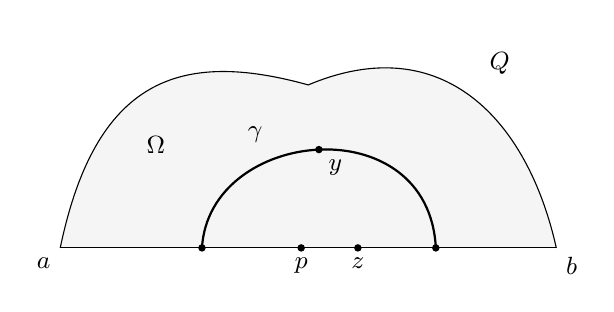
\begin{tikzpicture}[scale=.9, every node/.style={font=\small}]
  \coordinate (a) at (-3.5,0);
  \coordinate (b) at (3.5,0);
  \coordinate (p) at (-.1,0);
  \coordinate (z) at (.7,0);
  \coordinate (y) at (.15,1.3875);
  \fill[gray!8] (a)
    .. controls (-3,2.4) and (-1.8,2.8) .. (0,2.3)
    .. controls (1.9,3.1) and (3.1,1.8) .. (b)--cycle;
  \draw (a)--(b);
  \draw (a)
    .. controls (-3,2.4) and (-1.8,2.8) .. (0,2.3)
    .. controls (1.9,3.1) and (3.1,1.8) .. (b);
  \draw[thick] (-1.5,0)
    .. controls (-1.4,1.7) and (1.7,2) .. (1.8,0);
  \fill (-1.5,0) circle (1.5pt);
  \fill (1.8,0) circle (1.5pt);
  \fill (p) circle (1.5pt);
  \fill (z) circle (1.5pt);
  \fill (y) circle (1.5pt);
  \node[below left] at (a) {$a$};
  \node[below right] at (b) {$b$};
  \node[below] at (p) {$p$};
  \node[below] at (z) {$z$};
  \node[below right] at (y) {$y$};
  \node at (-.75,1.6) {$\gamma$};
  \node at (-2.15,1.45) {$\Omega$};
  \node at (2.7,2.6) {$Q$};
\end{tikzpicture}
\caption{The auxiliary Jordan disk and the level arc $\gamma$. The two
endpoints of $\gamma$ lie on $[a,b]$, on opposite sides of $p$;
$y$ and $z$ are the points selected in the proof. Only topological
incidences are shown. Distances are measured in the whole diagram;
shortest routes may leave $\Omega$ and are not drawn.}
\label{fig:level-arc}
\end{figure}

\subsection{Stability of controlled paths}

The next statement is the form of the classical Morse stability lemma
\cite[Chapter~III.H, Theorem~1.7, p.~401]{BH1999} needed to pass from diagram distances to
word distances. We include its
proof with constants suited to the present application. In its hypothesis, a subarc means a parameter
subinterval of the path; repetitions and retracing are allowed.

\begin{lemma}[Stability of paths with controlled subarc lengths]
\label{lem:path-stability}
Let $X$ be a geodesic metric space with $\delta$-thin geodesic triangles.
Fix $\lambda\ge1$ and $C\ge0$. There is $D=D(\delta,\lambda,C)$ such that
every rectifiable path $\sigma$ satisfying
\begin{equation}
 \operatorname{length}(\sigma|_{[u,v]})
 \le\lambda d(\sigma(u),\sigma(v))+C
 \quad\text{for every }u\le v
 \label{eq:all-subarc-bound}
\end{equation}
lies in the $D$-neighborhood of a geodesic $J$ with the same endpoints,
and $J$ lies in the $2D$-neighborhood of $\sigma$.
Consequently triangles whose three sides satisfy
\eqref{eq:all-subarc-bound} are $(3D+\delta)$-thin.
\end{lemma}

\begin{proof}
A point has a nearest point on $J$, because a geodesic segment is compact.
We first prove a projection estimate. Suppose $R_0>4\delta$,
$d(x,J),d(y,J)\ge R_0$, and $d(x,y)\le R_0/2$. Choose nearest points
$x',y'\in J$. Every point $z\in[x',y']\subset J$ is within $2\delta$
of one of the other three sides of the geodesic quadrilateral
$x,x',y',y$; a diagonal reduces this assertion to two thin triangles.
It cannot be within $2\delta$ of $w\in[x,y]$, for then
\[
 R_0\le d(x,J)\le d(x,z)
 \le d(x,w)+2\delta\le R_0/2+2\delta<R_0.
\]
If instead $d(z,w)\le2\delta$ for $w\in[x,x']$, nearest-point
minimality gives
\[
 d(x,x')\le d(x,z)\le d(x,w)+2\delta,
 \qquad d(w,x')\le2\delta,
\]
so $d(z,x')\le4\delta$. The analogous bound holds near $[y,y']$.
Thus every point of $[x',y']$ is within $4\delta$ of one of its
endpoints. Applying this to its midpoint proves
\begin{equation}
 d(x',y')\le8\delta.
 \label{eq:projection-contraction}
\end{equation}

Choose, for example, $R_0=1+32\lambda\delta$; then $R_0>4\delta$ and
$16\lambda\delta/R_0<1/2$. Every component of an excursion of $\sigma$
beyond distance $R_0$ from $J$ has both endpoints at distance $R_0$,
because the endpoints of the whole path belong to $J$. Let $H$ be the
length of its closure. Partition it by arclength into at most
$1+2H/R_0$ pieces of length at most $R_0/2$.
All partition points are at distance at least $R_0$ from $J$, so
\eqref{eq:projection-contraction}, summed over consecutive points,
bounds the distance between the projections of the excursion endpoints
by $8\delta(1+2H/R_0)$. Applying
\eqref{eq:all-subarc-bound} to the excursion gives
\begin{equation}
 H\le\lambda(2R_0+8\delta)
       +\frac{16\lambda\delta}{R_0}H+C.
 \label{eq:excursion-bound}
\end{equation}
Consequently $H\le2[\lambda(2R_0+8\delta)+C]$. Every point of the
excursion is within arclength $H/2$ of one of its endpoints. Hence the
whole path is within distance
\[
 D=R_0+\lambda(2R_0+8\delta)+C
\]
of $J$, including points outside the excursions.

For the reverse inclusion, let $s$ be the initial endpoint and fix
$q\in J$. By continuity along $\sigma$ there is a point $x\in\sigma$
with $d(s,x)=d(s,q)$. A nearest point $x'\in J$ satisfies
$d(x,x')\le D$, whence
\[
 d(q,x')=\bigl|d(s,q)-d(s,x')\bigr|
         =\bigl|d(s,x)-d(s,x')\bigr|\le D.
\]
Therefore $d(q,x)\le2D$. This uses the distance coordinate along the
fixed geodesic $J$, and requires no continuity of nearest-point choices.
Finally replace each side of a path triangle by a geodesic. A point on
one path is within $D$ of its geodesic, then within $\delta$ of another
geodesic, and then within $2D$ of the corresponding path.
\end{proof}

\subsection{Passage to word distance}

\begin{proposition}[Transfer to the Cayley graph]
\label{prop:word-hyperbolicity}
The group $G=\pi_1(K)$ is word-hyperbolic.
\end{proposition}

\begin{proof}
First compare the metric of a diagram with its graph metric. There is a
constant $B_1>0$, depending only on the fixed triangulation of $K$, such
that for diagram vertices $u,v$,
\begin{equation}
 d_{\Delta^{(1)},\mathrm{edges}}(u,v)\le B_1d_\Delta(u,v).
 \label{eq:diagram-edge-routing}
\end{equation}
Indeed a geodesic from $u$ to $v$ has finitely many straight pieces.
Replace each passage through a triangle interior by a route on its
boundary. For points on sides meeting at angle $\omega$, the route
through their common corner has length at most
$1/\sin(\omega/2)$ times their Euclidean distance: for radial lengths
$a,b$, the law of cosines gives
$|x-y|^2\ge(a+b)^2\sin^2(\omega/2)$.
For points on the same side use the side segment. Finitely many model
angles give one length factor $c\ge1$. Partial edge traversals in the
resulting graph path can be combined, deleting reversals, to give a
walk of full edges with no greater length. If $\ell_*>0$ is the minimum
model edge length, that walk uses at most
$c\,d_\Delta(u,v)/\ell_*$ edges. This proves
\eqref{eq:diagram-edge-routing}, also for diagrams with no faces.

Fix a vertex $o\in K$ and a spanning tree in its graph. Let $\tau_v$
be the tree path from $o$ to $v$. For every oriented edge $e:u\to v$,
take the element represented by $\tau_u e\tau_v^{-1}$, and let $S$ be
the finite symmetric set of its nonidentity values. These elements
generate $G$: every based edge loop factors into them by cancellation
of consecutive tree paths, and every loop has an edge-loop
representative. If $S$ is empty then $G$ is trivial and the assertion
is immediate. Otherwise choose one such based edge loop for each
$s\in S$, with the reverse loop for $s^{-1}$, and choose $B_2>0$
bounding all their metric lengths.

Consider a geodesic triangle with vertices in the Cayley graph
$\operatorname{Cay}(G,S)$. Expand its successive letters into the chosen
loops in $K$. The empty triangle is already thin. Otherwise their
concatenation is a nonempty nullhomotopic edge path and has a reduced
diagram. Mark each transition between letters on its
outside boundary walk. Thus each of the three boundary paths is
partitioned into letter loops of length at most $B_2$; its marks
correspond to the successive group vertices on its Cayley side.

For any two marks $u,v$ with group labels $g_u,g_v$,
\begin{equation}
 d_S(g_u,g_v)\le
 d_{\Delta^{(1)},\mathrm{edges}}(u,v)
 \le B_1d_\Delta(u,v).
 \label{eq:mark-displacement}
\end{equation}
To justify the first inequality, any diagram edge path from $u$ to $v$
has the same group displacement as the corresponding outside walk:
the two paths differ by an edge loop contractible in the diagram.
All marks map to $o$, and inserting the tree paths at successive target
vertices makes the displacement a product with at most one letter
of $S$ per edge. This argument also covers pinched boundary walks.
In particular, two marks which are the same diagram vertex have the
same group label. Distinct positions on a nonconstant geodesic Cayley
side therefore cannot become the same marked diagram vertex.

Between two marks on one side, the number of letters is precisely
their group distance, since that Cayley side is geodesic. Its expanded
subarc consequently has length at most
$B_2d_S(g_u,g_v)\le B_1B_2d_\Delta(u,v)$.
For an arbitrary parameter subarc from $x$ to $y$, extend to enclosing
marks $u,v$, adding at most $B_2$ at either end. With
\[
 \lambda=\max\{1,B_1B_2\},\qquad C=2\lambda B_2,
\]
we obtain
\[
 \operatorname{length}(x\text{ to }y)
 \le\lambda d_\Delta(u,v)
 \le\lambda d_\Delta(x,y)+2\lambda B_2.
\]
This bound holds even when a letter loop retraces edges or the two
subarc endpoints coincide in the diagram.

Lemmas~\ref{lem:diagram-thinness} and~\ref{lem:path-stability} now give
uniform thinness $T=3D+\delta$ for the expanded path triangle. A mark
on one side is within $T$ of some point on another side, hence within
$T+B_2$ of a mark on that side. By \eqref{eq:mark-displacement}, every
group vertex of a Cayley triangle is within
\[
 H_0=B_1(T+B_2)
\]
of a group vertex on another side. Every other point on a side is
within distance $1$ of a side vertex. Thus every geodesic triangle
whose corners are group vertices is $H$-thin, where $H=H_0+1$.

For completeness, this gives uniform thinness also when triangle
corners lie inside edges. A geodesic polygon with $n\ge3$ vertex
corners is $(n-2)H$-thin: draw geodesic diagonals from an endpoint of
the side under consideration and successively apply triangle thinness.
In an arbitrary geodesic triangle, keep on each side the segment
between its first and last graph vertices. If the side contains no
vertex, it is contained in one edge and has length less than $1$;
replace it by a constant segment at an endpoint of that edge.
Each kept or constant segment lies within distance $1$ of its original
side, and every discarded initial or final part has length at most
$1$. Join consecutive replacement segments by geodesics between their
vertex endpoints. Those endpoints are each within $1$ of the common
original corner, so every joining segment has length at most $2$.
This yields a six-sided vertex geodesic polygon, allowing constant
sides and repeated corners. The diagonal argument applies unchanged
to these degeneracies and gives thinness at most $4H$.
Each point of a joining side is within $1$ of its nearer endpoint,
hence within $2$ of the corresponding original corner. That corner
belongs to an original side other than any fixed side under
consideration. The other replacement segments either lie on their
original sides or are within distance $1$ of them. A point on a kept
segment is consequently within $4H+2$ of another original side.
Discarded tails are within $1$ of a shared corner; if an original side
has no vertices, every one of its points is within $1$ of its corners.
Thus $4H+2$ is a uniform thinness constant for all geodesic triangles
in the Cayley graph. This is word-hyperbolicity.
\end{proof}

Together with Propositions~\ref{prop:closed-paths} and~\ref{prop:no-torsion},
this proves Theorem~\ref{thm:triangle-complex} and completes the proof of
Theorem~\ref{thm:main}.


\bibliographystyle{plain}
\bibliography{references}
\end{document}
